\documentclass{article}

\usepackage[top=1in, bottom=1in, left=1.5in, right=1.5in, letterpaper]{geometry}
\usepackage{graphicx}
\usepackage{tikz}

\definecolor{pc1}{HTML}{8DD3C7}
\definecolor{pc2}{HTML}{FDB462}
\definecolor{pc3}{HTML}{FB8072}

\begin{document}

	\begin{figure*}[!htb]
		\centering
		\begin{tikzpicture}
			\node at (0, 0) {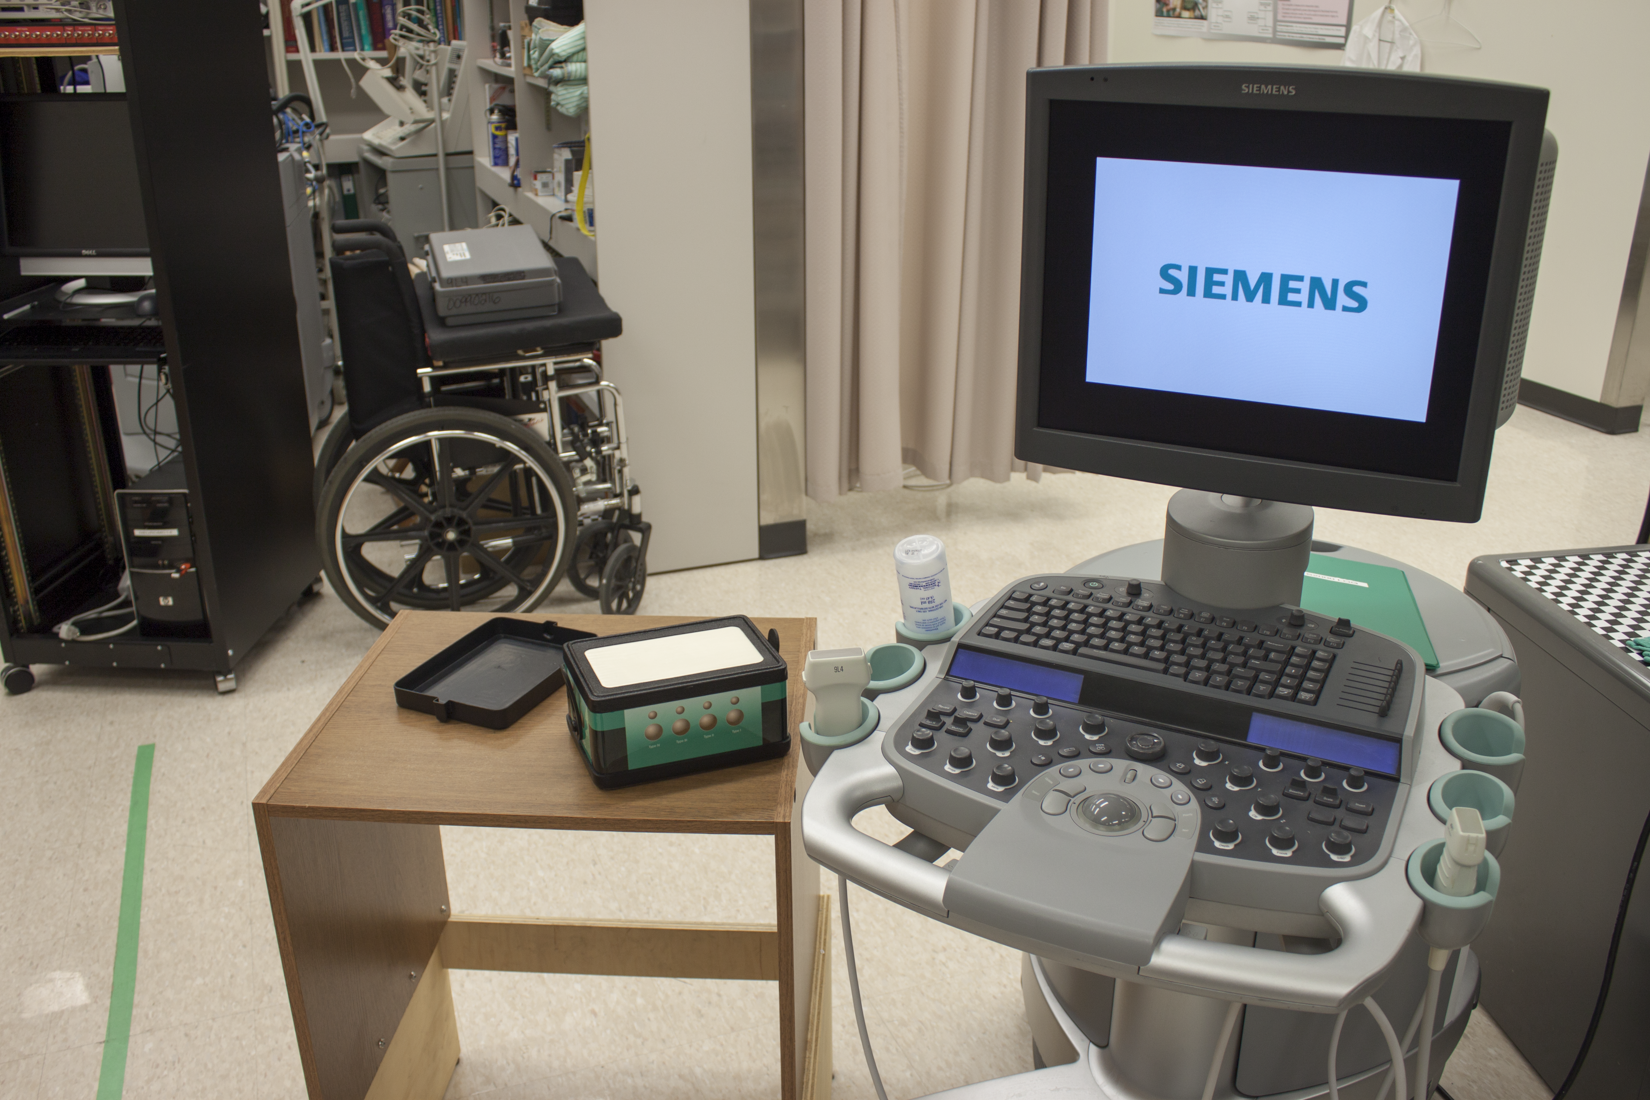
\includegraphics[width=\textwidth]{../assets/experimental_setup.png}};

			% the phantom
			\draw[pc1,->,ultra thick] (-0.5, 1) -- (-1,-0.9);
			\draw (-0.5, 1) node[above,text width=1in,align=center,fill=white,rounded corners=3pt,draw=pc1,ultra thick]{\color{black}CIRS Elasticity QA Phantom model 049};

			% the probe
			\draw[pc2,->,ultra thick] (-2, -3.15) -- (0, -1.3);
			\draw (-2, -3.15) node[below,text width=1in,align=center,fill=white,rounded corners=3pt,draw=pc2,ultra thick]{\color{black}9L4 Transducer};

			% the ultrasound machine
			\draw[pc3,->,ultra thick] (-0.5, 4) -- (2.5, 2.5);
			\draw (-0.5, 4) node[left,text width=1.5in,align=center,fill=white,rounded corners=3pt,draw=pc3,ultra thick]{\color{black}Siemens ACUSON S2000\textsuperscript{\texttrademark}\ portable ultrasound machine};
		\end{tikzpicture}
		\caption[]{Experimental setup showing the ultrasound machine, probe, and phantom model.}
		\label{fig:experimental_photo}
	\end{figure*}

\end{document}